\documentclass[../../main]{subfiles}

\renewcommand\thesection{\arabic{section}}


\begin{document}

\section{Core Block} \label{sec:}

As the name suggests, \emph{core block} is a crucially part of the thermal / exhaust system.
It has a three chambered design. A \emph{cooling chamber}, a \emph{heating chamber}, and
a \emph{common chamber}. These chambers are separated by panels. There's a total of seven
panels in the core block itself. Take a look at the figure \ref{fig:coreBlockParts} to
get a better grasp of the core block.

\begin{figure}
    \centering
    \includegraphics [
        max width = \IGXMaxWidth,
        max height = \IGXMaxHeight,
        \IGXDefaultOptionalArgs,
    ] {tikzpics/endCoreBlockPanels.pdf}
    \captionof{figure} {Core block and its components.}
    \label{fig:coreBlockParts}
\end{figure}

There's a pair of side panel, and a pair of bottom panel. Along with this there are three
middle panels. Unlike middle panels and bottom panels, side panels are half panels. When
each of them are open, they will expose the heating chamber and cooling chamber to the
outside. When they are closed\footnote{ie, covering the heating chamber or cooling chamber.},
the other side will still be closed.

\alertImportant{
    Middle and bottom panels are \emph{full} panels, meaning when the panel moves form one
    side to other, it opens one side and closes the other. Meanwhile side panels are
    \emph{half} panels, one side will always be closed, regardless of the state of the panel.
    In our case, both sides\footnote{left and right ends.} of the common chamber will always
    be closed.
}

Based on the state of these panels, the core block can be configured in different modes, each
of them serving different aspects of the thermal / exhaust system. These modes are, \emph{cooler
mode}, \emph{heater mode}, and \emph{exhaust mode}. This is achieved by selectively connecting
different chambers of the core block to the insides or the outsides of the Incubator. Following
sections will go through each of these modes.

\begin{center}
    \begin{minipage} {0.64\textwidth}

        Along with this, core block has three fans. These are unidirectional 12V DC brushless fans.
        Two for heating chamber and one for cooling chamber. All three of them are directed towards
        the heating and cooling sides of the peltier module, and are in the on state while the core
        block is either in cooler or heater modes. While the core block is in the exhaust mode, three
        of them are turned off. Figure \ref{fig:dc12VFan} shows that 12V fan we are using.

        Specification:

        \begin{itemize}
            \item \textbf{Operating voltage:} $12\si{V}$.
            \item \textbf{Operating current:} $220\si{mA}$.
        \end{itemize}

    \end{minipage}
    \hfill
    \begin{minipage} {0.35\textwidth}
        \centering
        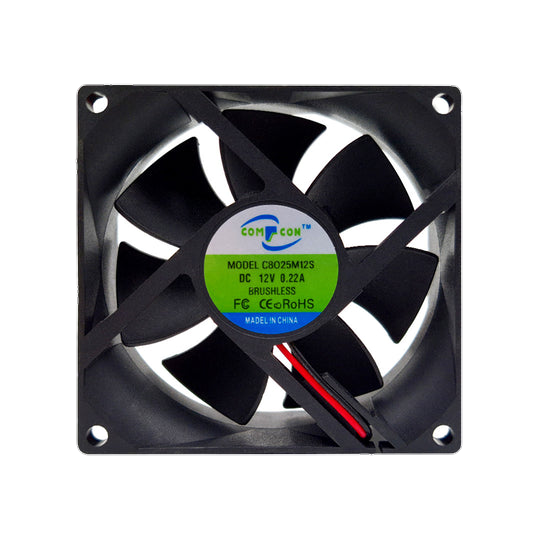
\includegraphics [
            height = 0.175\textheight,
            max width = \IGXMaxWidth,
            max height = \IGXMaxHeight,
            \IGXDefaultOptionalArgs,
            trim = {1cm 2cm 1cm 2cm},
            clip,
        ] {pics/fan.png}
        \captionof{figure} {DC brushless fan.}
        \label{fig:dc12VFan}
    \end{minipage}
\end{center}

\alertNote{

    % \begin{wrapfigure} {r} {0.49\textwidth}
    %     \vspace{-0.85cm}
    % \end{wrapfigure}

    Illustrations \ref{fig:coreBlockParts}, \ref{fig:coreBlockCMODE}, \ref{fig:coreBlockHMODE}, and
    \ref{fig:coreBlockEMODE} all are showing the top opened\footnote{of the common chamber.} version
    of the core block for better visibility of the insides. While operating, the core block's
    common chamber will be closed as shown in figure \ref{fig:coreBlockClosed}.

    \begin{center}
        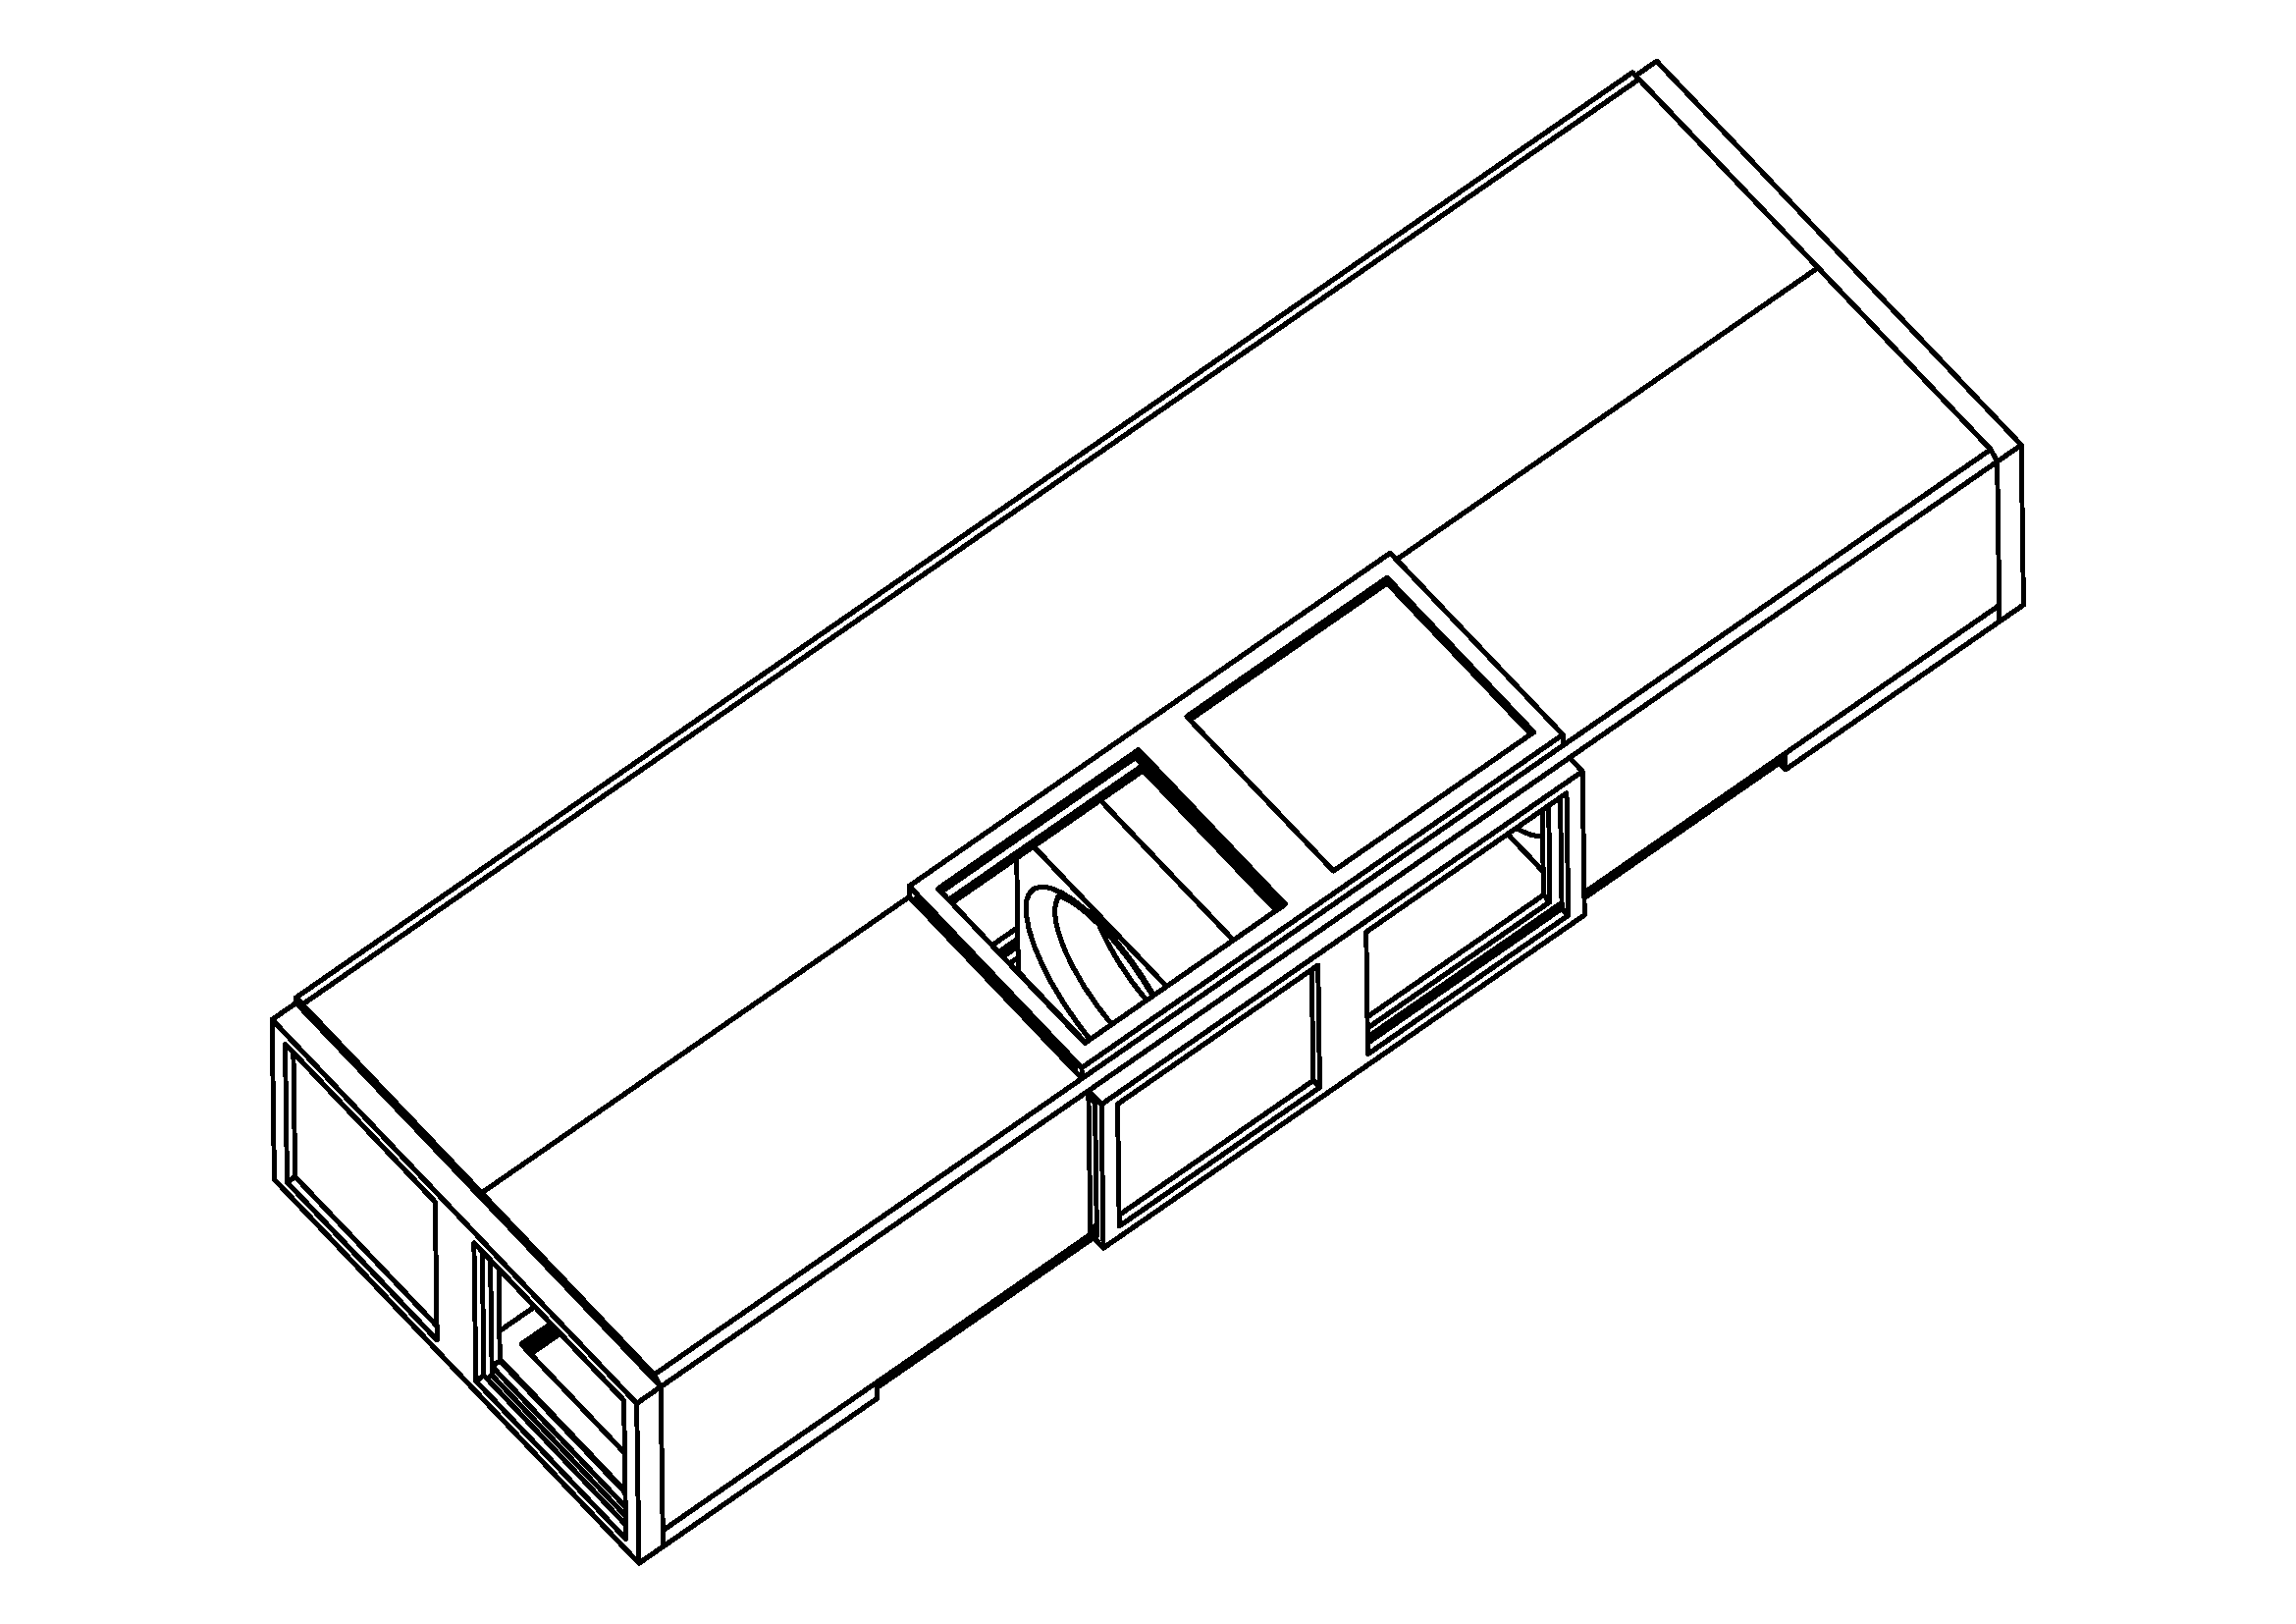
\includegraphics [
            width = 0.45\textwidth,
            max width = \IGXMaxWidth,
            max height = \IGXMaxHeight,
            \IGXDefaultOptionalArgs,
            trim = {4.5cm 0.0cm 4.5cm 1.0cm},
            clip,
        ] {pics/ortho_closed.pdf}
        \captionof{figure} {Closed off core block.}
        \label{fig:coreBlockClosed}
    \end{center}

}

\subsection{C Mode}

\texttt{CMODE} or cooler mode connects the cooling chamber with the common chamber and the incubator
insides. And disconnects the heating chamber from the incubator and connects it to the outsides. All
three fans are on and directed towards the peltier module. Heating chamber will pull the ambient air through
the right side and dissipates heat at the hotter side of the peltier module. The cooling chamber will
pull air from the incubator insides and cools it further and transfers it back to the incubator.
Figure \ref{fig:coreBlockCMODE} illustrates the state of panels in this mode.

\vfill

\begin{figure}
    \centering
    \includegraphics [
        max width = \IGXMaxWidth,
        max height = \IGXMaxHeight,
        \IGXDefaultOptionalArgs,
    ] {tikzpics/endCADExhaustCMODE.pdf}
    \captionof{figure} {Core block in \texttt{CMODE}.}
    \label{fig:coreBlockCMODE}
\end{figure}

\subsection{H Mode}

\texttt{HMODE} or heater mode connects the heating chamber with the common chamber and the incubator
insides. And disconnects the cooling chamber from the incubator and connects it to the outsides. All
three fans are on and directed towards the peltier module. Cooling chamber will pull the ambient air through
the left side and dissipates coldness at the cooler side of the peltier module. The heating chamber will
pull air from the incubator insides and heats it further and transfers it back to the incubator.
Figure \ref{fig:coreBlockHMODE} illustrates the state of panels in this mode.

\vfill

\begin{figure}
    \centering
    \includegraphics [
        max width = \IGXMaxWidth,
        max height = \IGXMaxHeight,
        \IGXDefaultOptionalArgs,
    ] {tikzpics/endCADExhaustHMODE.pdf}
    \captionof{figure} {Core block in \texttt{HMODE}.}
    \label{fig:coreBlockHMODE}
\end{figure}

\subsection{E Mode}

\texttt{EMODE} or exhaust mode disconnects the common chamber from the incubator and connects both the
cooling and heating chamber to both the outsides and the insides of the incubator. In this mode, all
three fans and peltier will be turned off. Figure \ref{fig:coreBlockHMODE} illustrates the state of panels
in this mode.

\vfill

\begin{figure}
    \centering
    \includegraphics [
        max width = \IGXMaxWidth,
        max height = \IGXMaxHeight,
        \IGXDefaultOptionalArgs,
    ] {tikzpics/endCADExhaustEMODE.pdf}
    \captionof{figure} {Core block in \texttt{EMODE}.}
    \label{fig:coreBlockEMODE}
\end{figure}


% \begin{figure}
%     \centering
% \end{figure}
%
% \begin{figure}
%     \centering
%     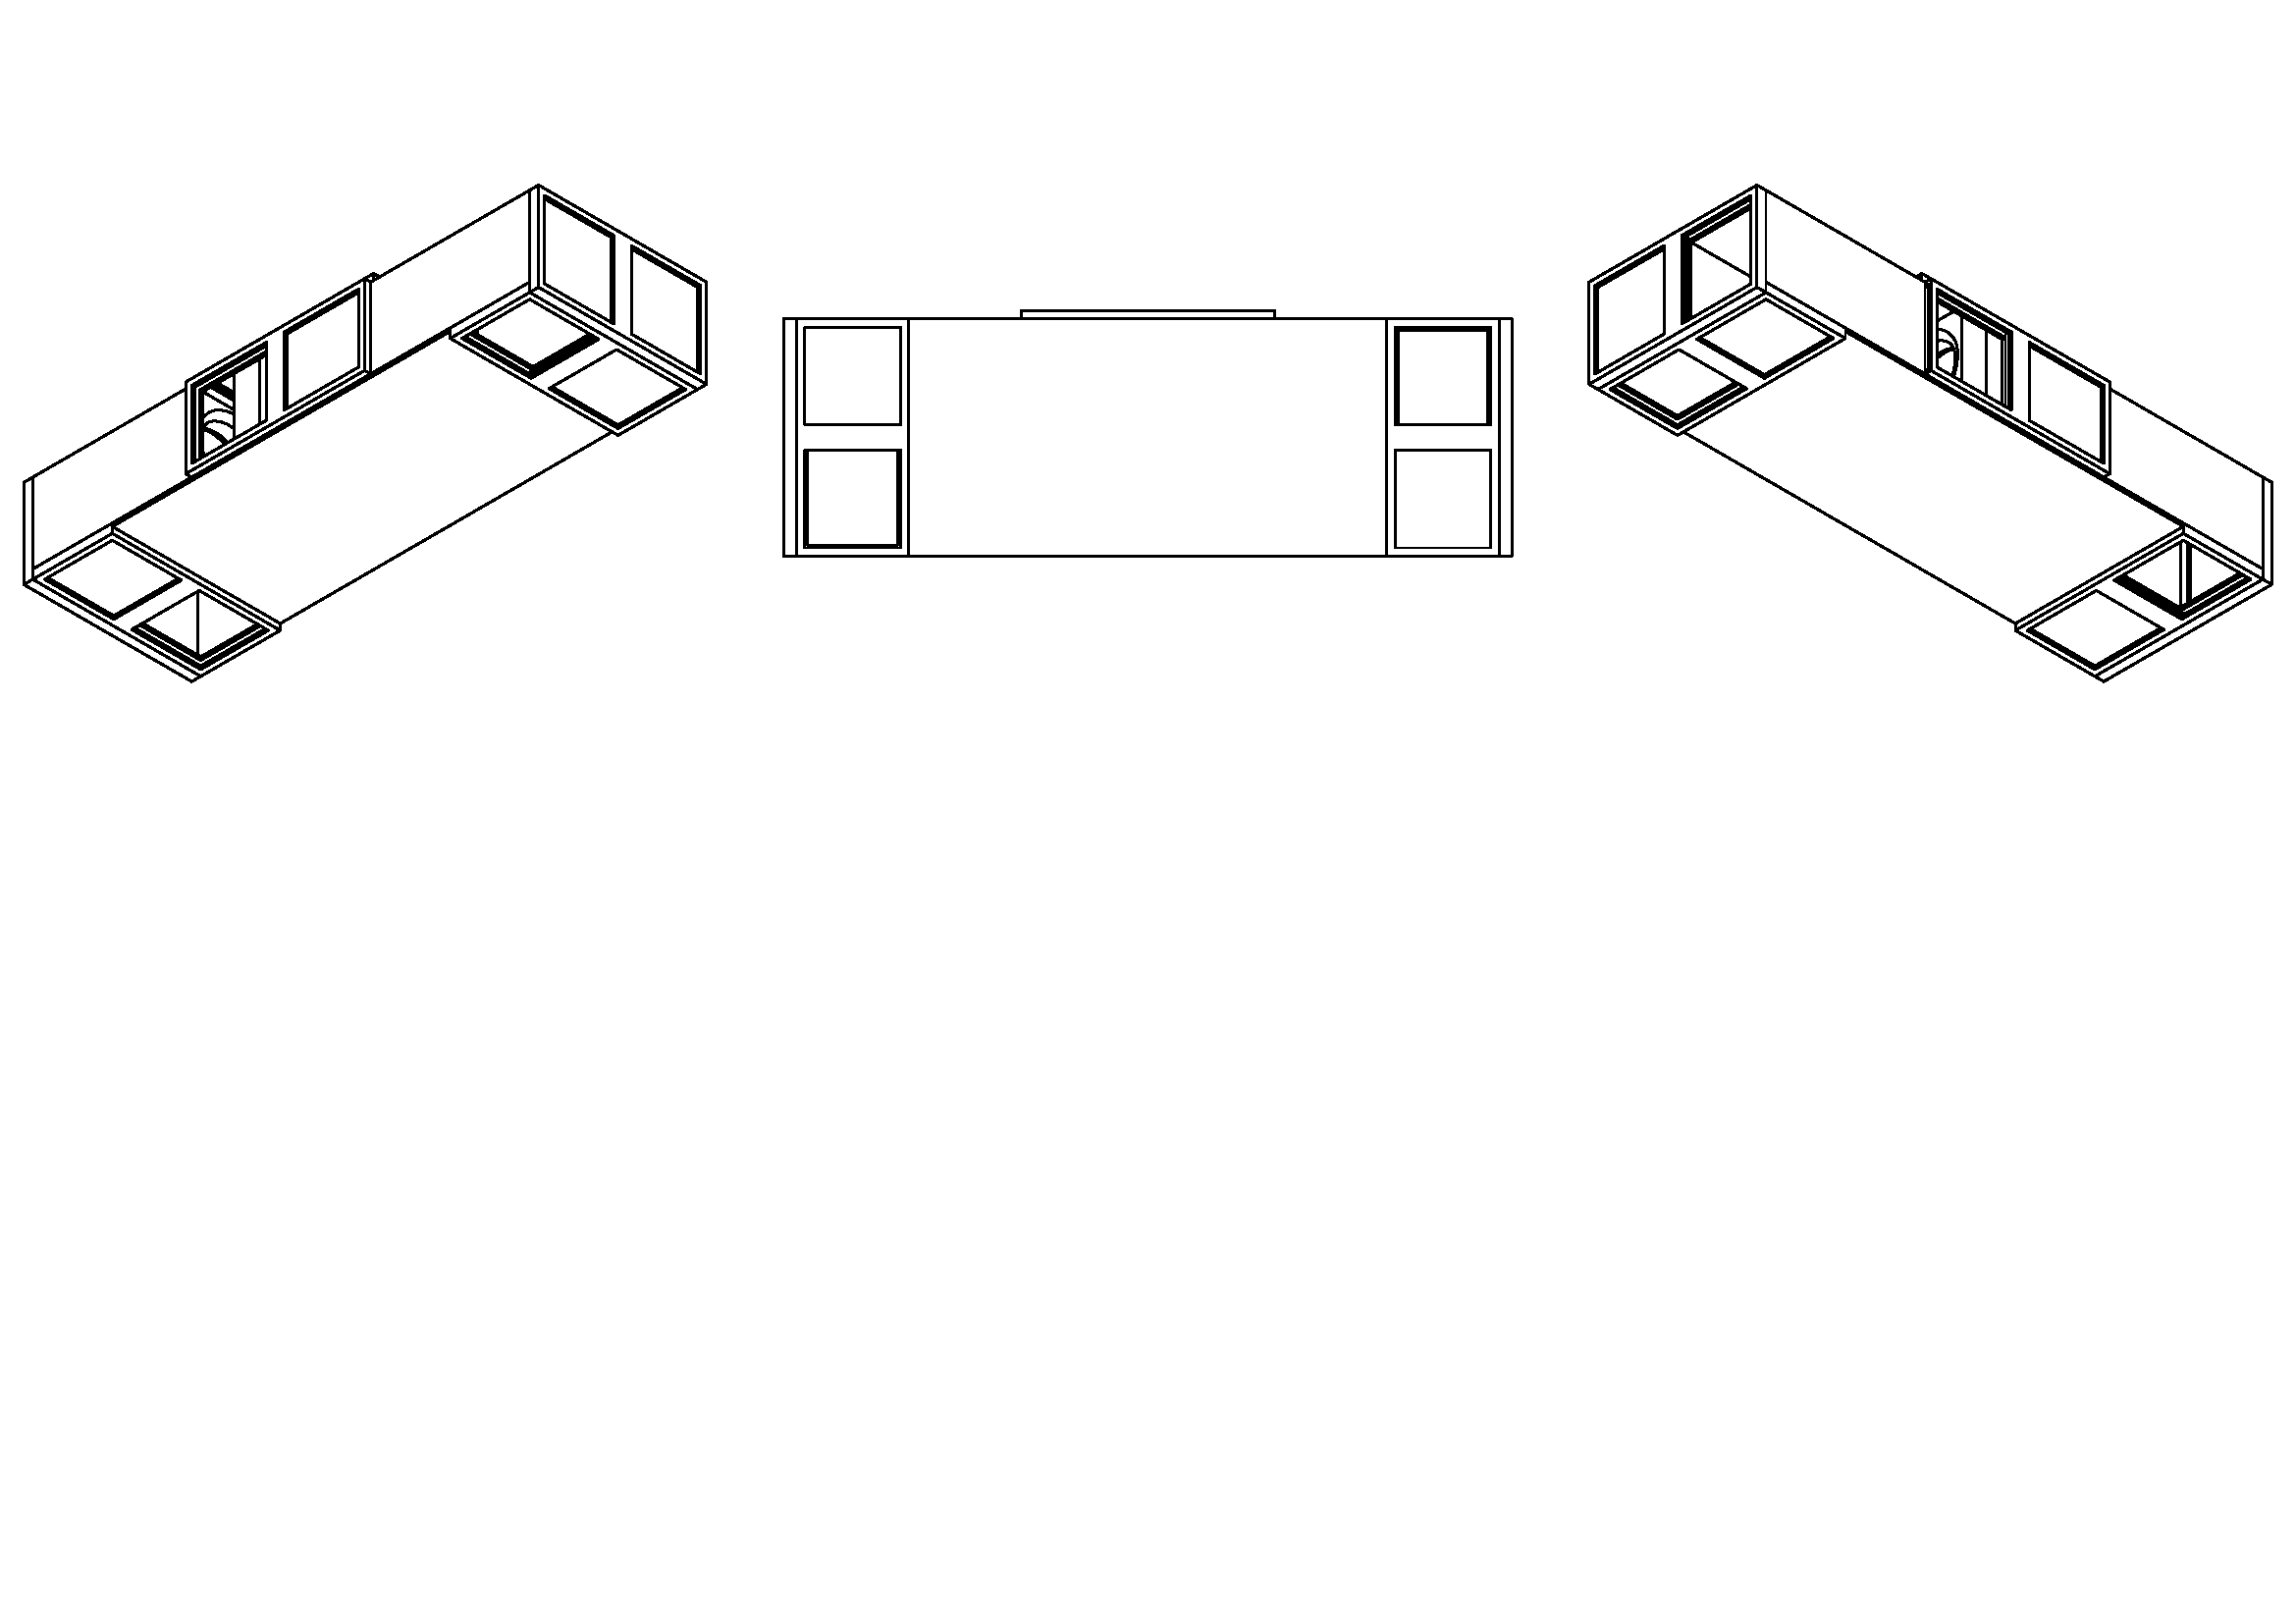
\includegraphics [
%         max width = \IGXMaxWidth,
%         max height = \IGXMaxHeight,
%         \IGXDefaultOptionalArgs,
%         trim = {0 16.25cm 0 3.15cm},
%         clip,
%     ] {pics/cmode_bot.pdf}
%     \captionof{figure} {}
%     \label{fig:}
% \end{figure}
%


\end{document}
